
\subsubsection{Analisi Derivazioni e Ridondanze}

\paragraph[H]{Attributo Difesa}L'unico dato derivabile che viene utilizzato dalle nostre operazione  la Difesa del Personaggio (operazioni 13,14,19,20,46). L'attributo in questione pu\`{o} essere ricavato dalla somma della difesa degli oggetti indossati e dalla somma della difesa delle occorrenze dell'entit\`{a} consumo. Di seguito si valuta la convenienza di utilizzo del dato difesa.



\begin{table}[H]
\centering
\caption{Operazione 13}
\begin{tabular}{llll}
\\ \hline
\multicolumn{1}{|l|}{\textbf{CONCETTO}} & \multicolumn{1}{l|}{\textbf{COSTRUTTO}} & \multicolumn{1}{l|}{\textbf{ACCESSI}} & \multicolumn{1}{l|}{\textbf{TIPO}} \\ \hline
\multicolumn{1}{|l|}{Indossamento}      & \multicolumn{1}{l|}{R}                  & \multicolumn{1}{l|}{1}                & \multicolumn{1}{l|}{L}             \\ \hline
\multicolumn{1}{|l|}{Stock}             & \multicolumn{1}{l|}{R}                  & \multicolumn{1}{l|}{1}                & \multicolumn{1}{l|}{L}             \\ \hline
\multicolumn{1}{|l|}{Indossamento}      & \multicolumn{1}{l|}{R}                  & \multicolumn{1}{l|}{2}                & \multicolumn{1}{l|}{S}             \\ \hline
\multicolumn{1}{|l|}{Stock}             & \multicolumn{1}{l|}{R}                  & \multicolumn{1}{l|}{2}                & \multicolumn{1}{l|}{S}             \\ \hline
\end{tabular}
\end{table}


\begin{table}[H]
\centering
\caption{Operazione 14}
\label{my-label}
\begin{tabular}{|l|l|l|l|}
\hline
\textbf{CONCETTO} & \textbf{COSTRUTTO} & \textbf{ACCESSI} & \textbf{TIPO} \\ \hline
Consumo           & E                  & 1                & S             \\ \hline
Consumante        & R                  & 1                & S             \\ \hline
Consunto          & R                  & 1                & S             \\ \hline
\end{tabular}
\end{table}


\begin{table}[H]
\centering
\caption{Operazione 19}
\label{my-label}
\begin{tabular}{|l|l|l|l|}
\hline
\textbf{CONCETTO} & \textbf{COSTRUTTO} & \textbf{ACCESSI} & \textbf{TIPO} \\ \hline
Personaggio       & E                  & 1                & L             \\ \hline
Equipaggiamento   & E                  & 1                & L             \\ \hline
Indossamento      & R                  & 1                & S             \\ \hline
\end{tabular}
\end{table}

\begin{table}[H]
\centering
\caption{Operazione 20}
\label{my-label}
\begin{tabular}{|l|l|l|l|}
\hline
\textbf{CONCETTO} & \textbf{COSTRUTTO} & \textbf{ACCESSI} & \textbf{TIPO} \\ \hline
Consumo           & E                  & 1                & L             \\ \hline
Consumo           & E                  & 1                & S             \\ \hline
\end{tabular}
\end{table}


\begin{table}[H]
\centering
\caption{Operazione 46}
\label{my-label}
\begin{tabular}{|l|l|l|l|}
\hline
\textbf{CONCETTO} & \textbf{COSTRUTTO} & \textbf{ACCESSI} & \textbf{TIPO} \\ \hline
Consunto          & R                  & 1                & L             \\ \hline
Consumabili       & E                  & 1                & L             \\ \hline
Consumo           & E                  & 1                & L             \\ \hline
\end{tabular}
\end{table}




\begin{table}[H]
\centering
\caption{Operazione 13}
\label{my-label}
\begin{tabular}{|l|l|l|l|}
\hline
\textbf{CONCETTO} & \textbf{COSTRUTTO} & \textbf{ACCESSI} & \textbf{TIPO} \\ \hline
Indossamento      & R                  & 1                & L             \\ \hline
Stock             & R                  & 1                & L             \\ \hline
Indossamento      & R                  & 2                & S             \\ \hline
Stock             & R                  & 2                & S             \\ \hline
Personaggio       & E                  & 1                & L             \\ \hline
Personaggio       & E                  & 1                & L             \\ \hline
\end{tabular}
\end{table}



\begin{table}[H]
\centering
\caption{Operazione 14}
\label{my-label}
\begin{tabular}{|l|l|l|l|}
\hline
\textbf{CONCETTO} & \textbf{COSTRUTTO} & \textbf{ACCESSI} & \textbf{TIPO} \\ \hline
Consumo           & E                  & 1                & S             \\ \hline
Consumante        & R                  & 1                & S             \\ \hline
Consunto          & R                  & 1                & S             \\ \hline
Personaggio       & E                  & 1                & L             \\ \hline
Personaggio       & E                  & 1                & L             \\ \hline
\end{tabular}
\end{table}


\begin{table}[H]
\centering
\caption{Operazione 19}
\label{my-label}
\begin{tabular}{|l|l|l|l|}
\hline
\textbf{CONCETTO} & \textbf{COSTRUTTO} & \textbf{ACCESSI} & \textbf{TIPO} \\ \hline
Personaggio       & E                  & 1                & L             \\ \hline
Equipaggiamento   & E                  & 1                & L             \\ \hline
Indossamento      & R                  & 1                & S             \\ \hline
Personaggio       & E                  & 1                & L             \\ \hline
Personaggio       & E                  & 1                & L             \\ \hline
\end{tabular}
\end{table}


\begin{table}[H]
\centering
\caption{Operazione 20}
\label{my-label}
\begin{tabular}{|l|l|l|l|}
\hline
\textbf{CONCETTO} & \textbf{COSTRUTTO} & \textbf{ACCESSI} & \textbf{TIPO} \\ \hline
Consumo           & E                  & 1                & L             \\ \hline
Consumo           & E                  & 1                & S             \\ \hline
Personaggio       & E                  & 1                & L             \\ \hline
Personaggio       & E                  & 1                & L             \\ \hline
\end{tabular}
\end{table}

\begin{table}[H]
\centering
\caption{Operazione 46}
\label{my-label}
\begin{tabular}{|l|l|l|l|}
\hline
\textbf{CONCETTO} & \textbf{COSTRUTTO} & \textbf{ACCESSI} & \textbf{TIPO} \\ \hline
Consunto          & R                  & 1                & L             \\ \hline
Consumabili       & E                  & 1                & L             \\ \hline
Consumo           & E                  & 1                & L             \\ \hline
Personaggio       & E                  & 1                & L             \\ \hline
Personaggio       & E                  & 1                & L             \\ \hline
\end{tabular}
\end{table}




\begin{table}[H]
\centering
\caption{Costo Operazioni senza ridondanza}
\label{my-label}
\resizebox{\textwidth}{!}{%
\begin{tabular}{|l|l|l|l|}
\hline
\textbf{OPERAZIONE}               & \textbf{COSTO} & \textbf{FREQUENZA} & \textbf{TOTALE} \\ \hline
13                                & 10             & 100000             & 1000000         \\ \hline
14                                & 6              & 87500              & 525000          \\ \hline
19                                & 4              & 100000             & 400000          \\ \hline
20                                & 3              & 87500              & 262500          \\ \hline
46                                & 3              & 100000             & 300000          \\ \hline
COSTO OPERAZIONI SENZA RIDONDANZA & \hl{2487500}        &                    &                 \\ \hline
\end{tabular}
}
\end{table}

\begin{table}[H]
\centering
\caption{Costo Operazioni con Ridondanza}
\label{my-label}
\resizebox{\textwidth}{!}{%
\begin{tabular}{|l|l|l|l|}
\hline
\textbf{OPERAZIONE}             & \textbf{COSTO} & \textbf{FREQUENZA} & \textbf{TOTALE} \\ \hline
13                              & 13             & 100000             & 1300000         \\ \hline
14                              & 9              & 87500              & 787500          \\ \hline
19                              & 7              & 100000             & 700000          \\ \hline
20                              & 6              & 87500              & 525000          \\ \hline
46                              & 6              & 100000             & 600000          \\ \hline
COSTO OPERAZIONI CON RIDONDANZA & \hl{3912500}        &                    &                 \\ \hline
\end{tabular}
}
\end{table}

Alla luce della di quanto visto precedentemente abbiamo riscontrato un aumento del costo delle operazioni con la Ridondanza di circa il 40\%, si rende quindi necessario eliminare tale Dato.



\subsubsection{Eliminazione Delle Gerarchie}

Nel nostro schema concettuale sono presenti 3 generalizzazioni. Le Entità coinvolte sono Prodotto, oggetto ed NPC abbiamo deciso di procedere nel seguente modo:

\paragraph{Prodotto}
Per il prodotto abbiamo mantenuto i Figli e il padre in quanto entrambi erano coinvolti in relazioni, soprattutto il padre, cosa che avrebbe comportato una duplicazione di molte relazioni.
\paragraph{Oggetto} 
Anche per l'Oggetto abbiamo mantenuto i Figli e il padre in quanto entrambi erano coinvolti in relazioni e avrebbe comportato una duplicazione di molte relazioni.
\paragraph{NPC}Per gli NPC abbiamo deciso di accorpare il Genitore della Generalizzazione nei Figli, questo perchè quasi la totalità delle operazioni si riferiscono alle occorrenze dei figli.
Questa scelta comporta un risparmio notevole di Memoria rispetto alle alternative.



\newpage


\begin{landscape} %inizia un foglio landscape

%include un file pdf che contiene lo schema 
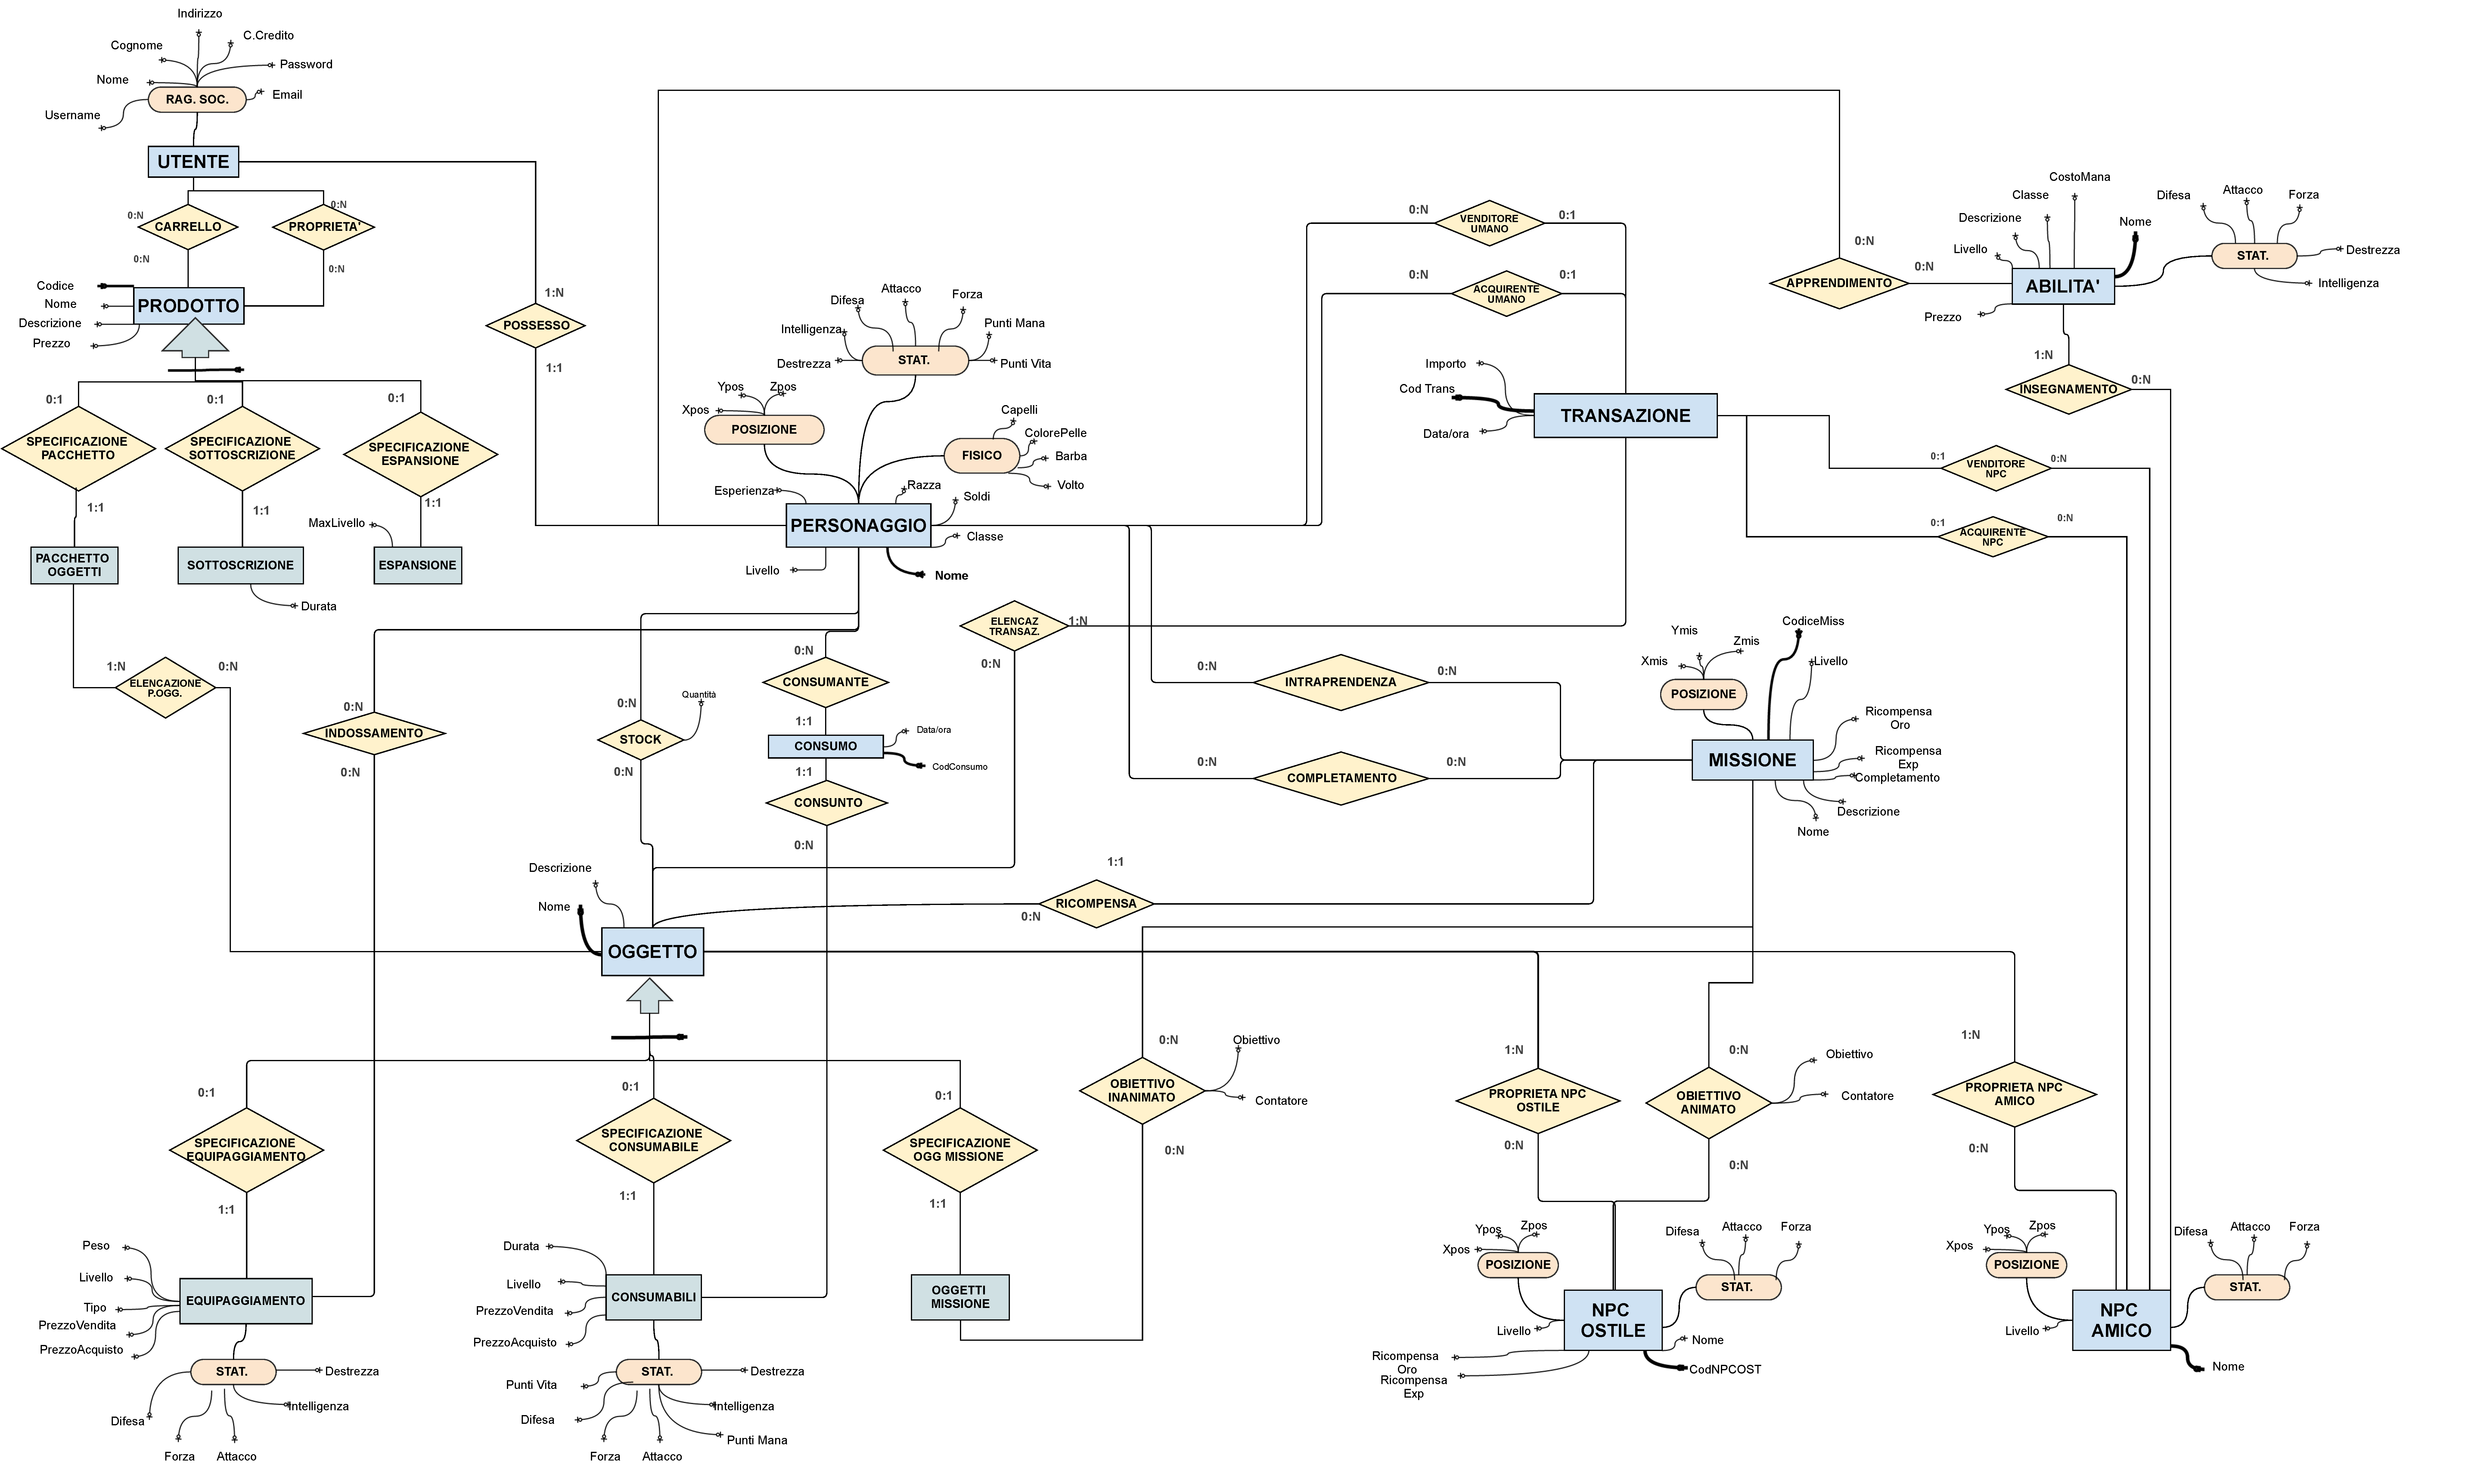
\includepdf[width=270mm, height=210mm, angle=90, keepaspectratio]{./pdf/ristrutturatosenzacarta.pdf}

\end{landscape}



\subsubsection{Eliminazione Attributi Multivalore}

Abbiamo individuato un attributo multivalore nella Carta di Credito e abbiamo eseguito una ristrutturazione


\begin{figure}[H]
\centering
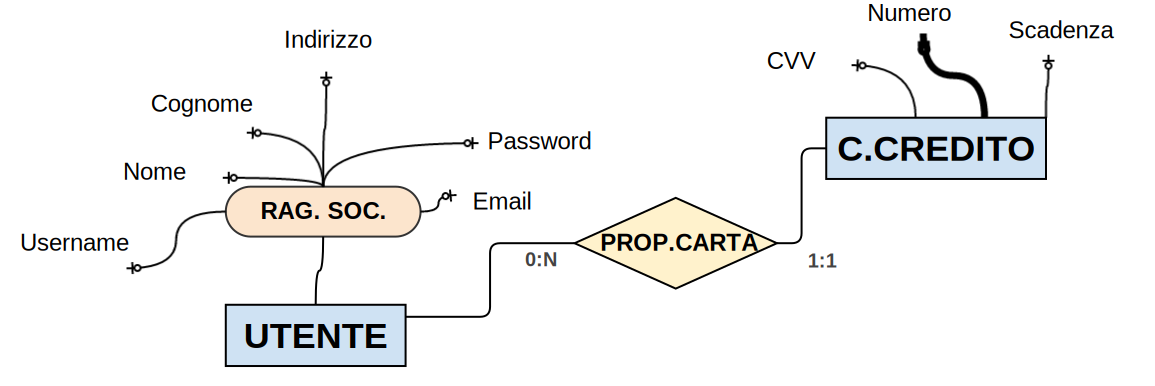
\includegraphics[width=0.7\linewidth]{./immagini/schemetto}
\caption{}
\label{fig:schemetto}
\end{figure}


